\subsection{Señalamiento original}

    El señalamiento original, ilustrado en la Figura \ref{fig:EJ6_2}, incluye señales de parada próximas a los finales de vías absolutos (S11, S12, S13, S14, S16), señales de maniobras antes de converger en una vía principal (S10, S15, S20) y señales múltiples para cambios de vías divergentes (S01, S06, S07, S21), entre varias otras señales.
    
    \begin{figure}[H]
    	\centering
    	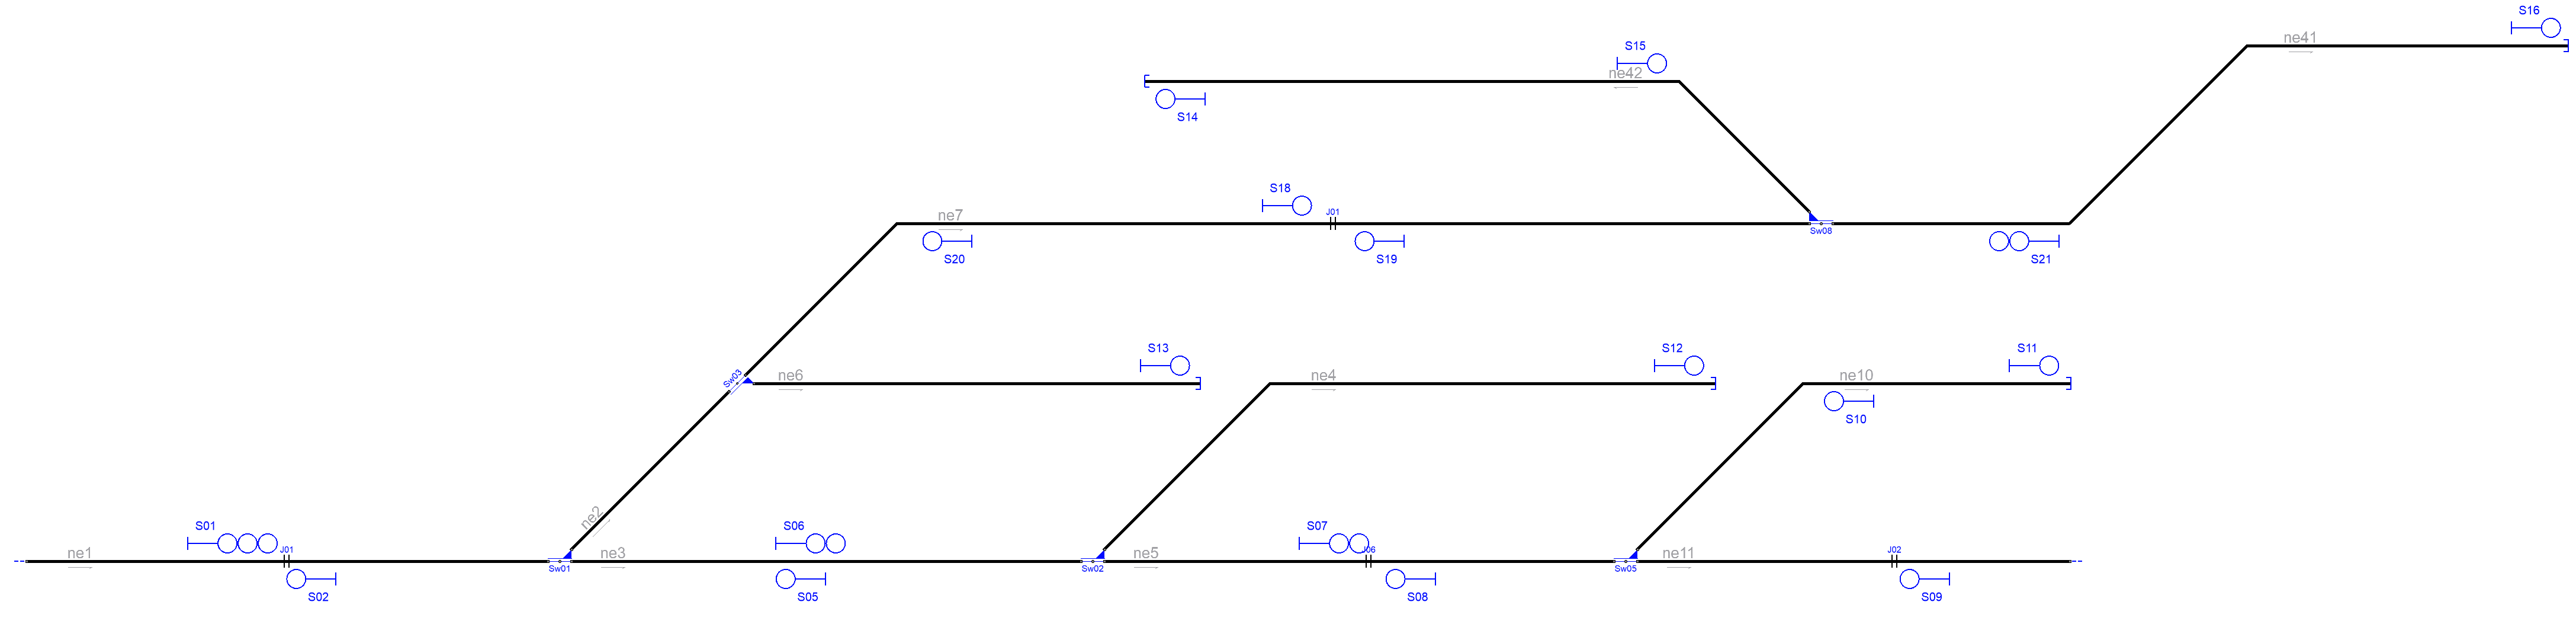
\includegraphics[width=1\textwidth]{resultados-obtenidos/ejemplo6/images/6_original.png}
    	\centering\caption{Señalamiento original del ejemplo 6.}
    	\label{fig:EJ1_2}
    \end{figure}
    
    Estas señales permiten definir hasta un máximo de 16 rutas, todas ellas detalladas en la Tabla \ref{Tab:tabla_original_6}. En una primera inspección, se puede comprobar que todos los elementos ferroviarios son alcanzados por al menos una de las rutas, en al menos una dirección. Además, todos los cambios de vías son utilizados, de forma simple o compuesta. 
    
    \begin{table}[H]
        {
        \caption{Tabla de enclavamiento original del ejemplo 6.}
        \label{Tab:tabla_original_6}
        \centering
        \resizebox{1\textwidth}{!}{
            \begin{tabular}{ c c c c c c c }
                \hline	
                    Ruta & Inicio & Final & Cambio & Plataforma & Cruce & netElement \\	
                \hline
                    R$_{01}$  & S$_{01}$ & S$_{06}$ & Sw$_{01}^{N}$ & - & - & ne$_{01}$-ne$_{03}$\\
                    R$_{02}$  & S$_{01}$ & S$_{13}$ & Sw$_{01}^{R}$+Sw$_{03}^{R}$ & - & - & ne$_{01}$-ne$_{06}$\\
                    R$_{03}$  & S$_{01}$ & S$_{18}$ & Sw$_{01}^{R}$+Sw$_{03}^{R}$ & - & - & ne$_{01}$-ne$_{07}$\\
                    R$_{04}$  & S$_{06}$ & S$_{07}$ & Sw$_{02}^{N}$ & - & - & ne$_{03}$-ne$_{05}$\\
                    R$_{05}$  & S$_{06}$ & S$_{12}$ & Sw$_{02}^{R}$ & - & - & ne$_{03}$-ne$_{04}$\\
                    R$_{06}$  & S$_{21}$ & S$_{19}$ & Sw$_{08}^{N}$ & - & - & ne$_{41}$-ne$_{07}$\\
                    R$_{07}$  & S$_{21}$ & S$_{14}$ & Sw$_{08}^{R}$ & - & - & ne$_{41}$-ne$_{42}$\\
                    R$_{08}$  & S$_{05}$ & S$_{02}$ & Sw$_{01}^{N}$ & - & - & ne$_{03}$-ne$_{01}$\\
                    R$_{09}$  & S$_{09}$ & S$_{08}$ & Sw$_{05}^{N}$ & - & - & ne$_{11}$-ne$_{05}$\\
                    R$_{10}$  & S$_{08}$ & S$_{05}$ & Sw$_{02}^{N}$ & - & - & ne$_{05}$-ne$_{03}$\\
                    R$_{11}$  & S$_{10}$ & S$_{08}$ & Sw$_{05}^{R}$ & - & - & ne$_{10}$-ne$_{05}$\\
                    R$_{12}$  & S$_{15}$ & S$_{16}$ & Sw$_{08}^{R}$ & - & - & ne$_{42}$-ne$_{41}$\\
                    R$_{13}$  & S$_{18}$ & S$_{16}$ & Sw$_{08}^{N}$ & - & - & ne$_{07}$-ne$_{41}$\\
                    R$_{14}$  & S$_{19}$ & S$_{20}$ & - & - & - & ne$_{07}$\\
                    R$_{15}$  & S$_{20}$ & S$_{02}$ & Sw$_{01}^{R}$+Sw$_{03}^{N}$ & - & - & ne$_{07}$-ne$_{01}$\\
                    R$_{16}$  & S$_{07}$ & S$_{11}$ & Sw$_{05}^{R}$ & - & - & ne$_{05}$-ne$_{10}$\\
                \hline
            \end{tabular}
        }
     }
    \end{table}
    
    Algunas rutas abarcan mas de un \textit{netElement}, como por ejemplo la ruta R15 que comienza en la señal S20 y finaliza en la señal S02, atravesando los \textit{netElements} ne07 y ne01, utilizando los cambios de vías Sw01 y Sw03, en posición reversa y normal respectivamente.